%!TEX encoding = UTF-8 Unicode
% -*- coding: UTF-8; -*-
% vim: set fenc=utf-8
\documentclass[12pt, ULlof, ULlot]{ULrapport}

\usepackage[utf8]{inputenc}
\usepackage[autolanguage]{numprint}
\usepackage[french]{babel}
\usepackage{icomma}
\usepackage{graphicx}
\usepackage{amsmath}
\usepackage{hyperref}
\usepackage{multirow}
\usepackage{array}
\usepackage{afterpage}
\usepackage{longtable}
\usepackage{booktabs}

\makeatletter
\newcommand{\thickhline}{%
    \noalign {\ifnum 0=`}\fi \hrule height 1pt
    \futurelet \reserved@a \@xhline
}
\newcommand{\e}[1]{\ensuremath{\times 10^{#1}}}
\newcommand{\degree}{\ensuremath{^\circ}}
\newcolumntype{"}{@{\hskip\tabcolsep\vrule width 1pt\hskip\tabcolsep}}
\makeatother

%Cette ligne permet de changer le nom d'un tableau : il change «Table x.x» (anglais) pour «Tableau x.x» (français). La classe ULrapport est suppose le faire, mais ne le fait pas.
\addto\captionsfrench{\def\tablename{{\sc{Tableau}}}}

\setlength\parskip{\baselineskip}

\TitreProjet{VisuaLigue (VL)}
\TitreRapport{Rapport de projet -- version 1.0}
\Destinataire{Martin Savoie, Jonathan Gaudreault}
\NumeroEquipe{01}
\NomEquipe{GIFTW}
\TableauMembres{%
        111\,099\,643 & Alexandre Gingras-Courchesne &\\\hline
        111\,106\,456 & Jérôme Isabelle &\\\hline
        111\,107\,781 & Maxime Ménard &\\\hline
        111\,098\,395 & Alexandra Mercier &\\\hline
}

\DateRemise{2 octobre 2016}

\HistoriqueVersions{%
    0.0 & 18 septembre 2016 & Création du document \\\hline
    1.0 & 2 octobre 2016 & Première remise \\\hline
    2.0 & 6 novembre 2016 & Livrable 2\\\hline
}

%Corps du document

\begin{document}

% Chapitres
%!TEX encoding = UTF-8 Unicode
% -*- coding: UTF-8; -*-
% vim: set fenc-utf-8

\chapter{Diagrammes de classe de conception}
\label{s:classe_conception}

Ce chapitre présente les différents diagrammes de classe de conception de \textit{VisualLigue}.

La figure \ref{fig:vue_classes_conception_diag} présente le diagramme de classes de la couche présentation(vue).
Puisque la technologie JavaFX est utilisée en union avec le constructeur d'interface graphique \textit{Scene Builder}, chaque classe représente un contrôleur pour une partie de la vue.
Il y a donc un fichier FXML associé à chacune de ces classes qui contient le code des éléments graphiques.
De prime abord, la classe \textit{RootLayoutController} représente la fenêtre de base de l'application.
Celle-ci contient la barre de menu principal, permet d'exécuter la majorité des fonctionnalités du logiciel.
C'est pour cela que ce contrôleur contient une majorité des méthodes permettant la gestion des événements.
Par ailleurs, le patron de conception \textit{Observateur} est utilisé afin de rediriger la gestion de certains événements vers le \textit{RootLayoutController}.
Cela permet d'éviter une duplication du code de gestion des événements tout en maintenant le couplage bas.
Ainsi, la même fonctionnalité peut être exécutée par la barre de menu ou par un bouton dans un autre contrôleur.


%\begin{figure}[htpb]
    %\centering
    %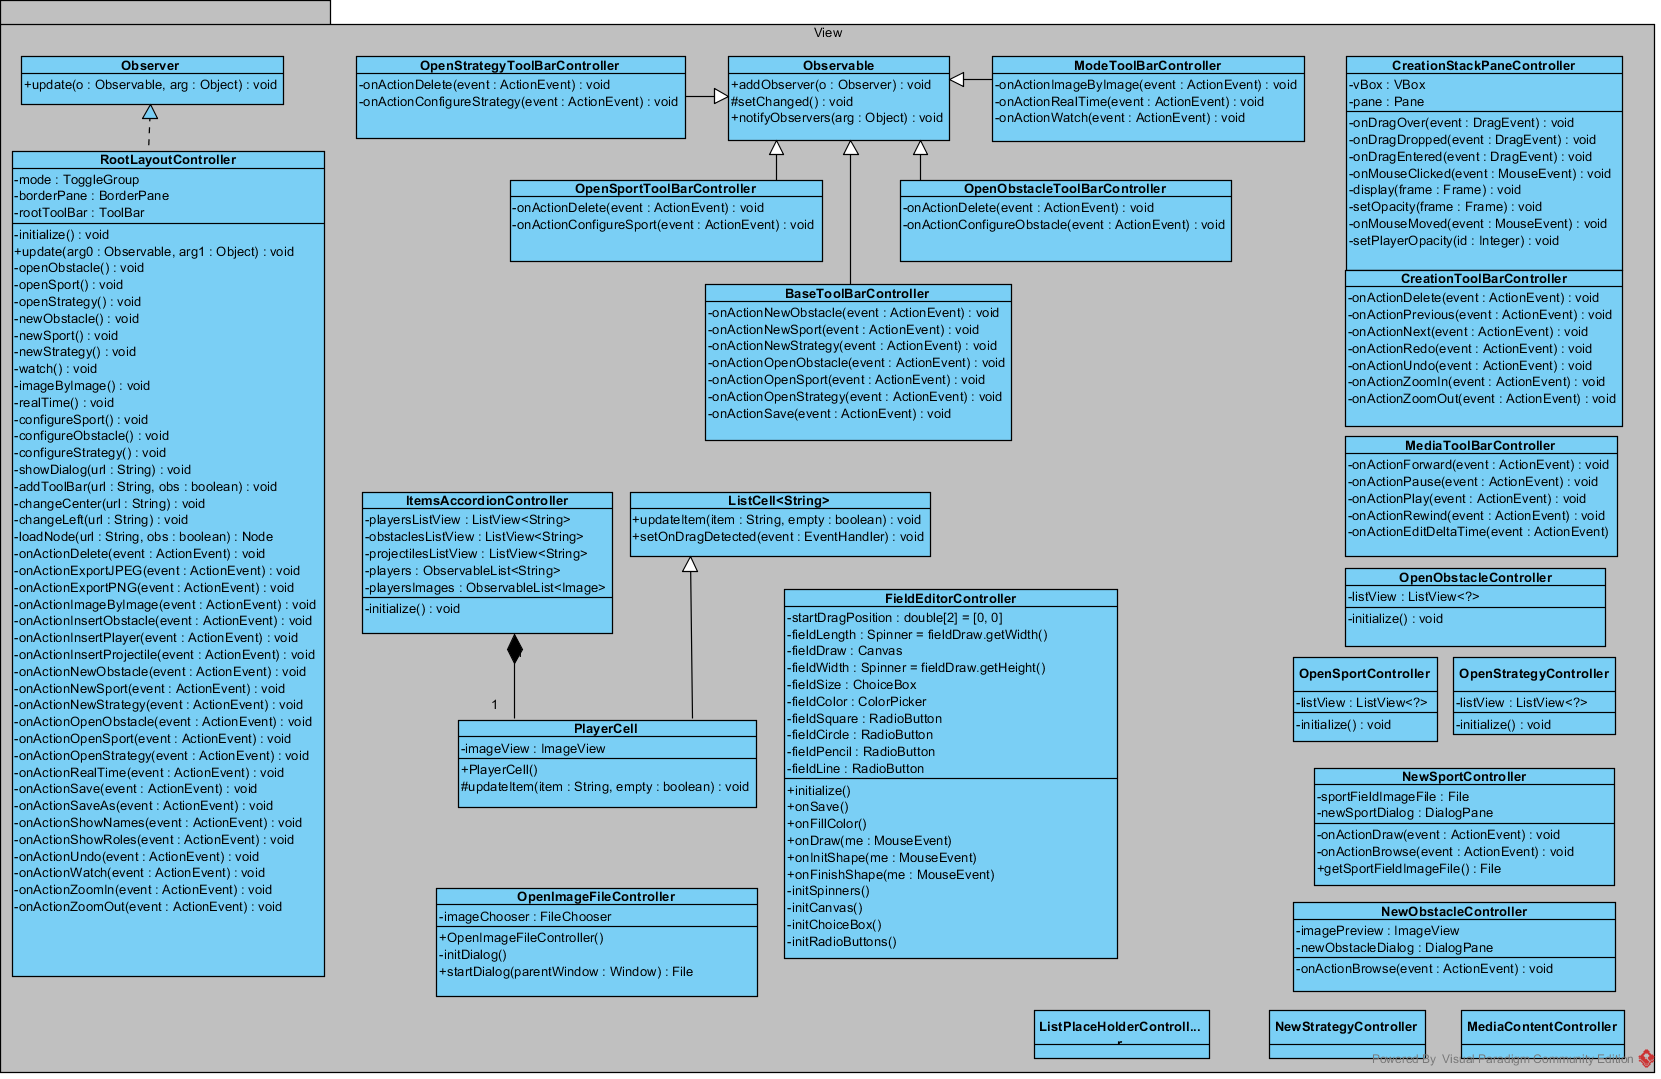
\includegraphics[scale=0.6]{fig/vue_classes_conception_diag.png}
    %\caption{Diagramme de classes de conception de la couche présentation}
    %\label{fig:vue_classes_conception_diag}
%\end{figure}
%!TEX encoding = UTF-8 Unicode
% -*- coding: UTF-8; -*-
% vim: set fenc-utf-8

\chapter{Diagrammes de séquence de conception}
\label{s:sequence_conception}

Ce chapitre présente les diagrammes de séquence de conception associée aux fonctionnalitées de l'application.

\section{Convertir les coordonnées de la souris en coordonnées réelles}
\label{sec:convertir_coordonnees_souris}

%\begin{figure}[htpb]
%    \centering
%    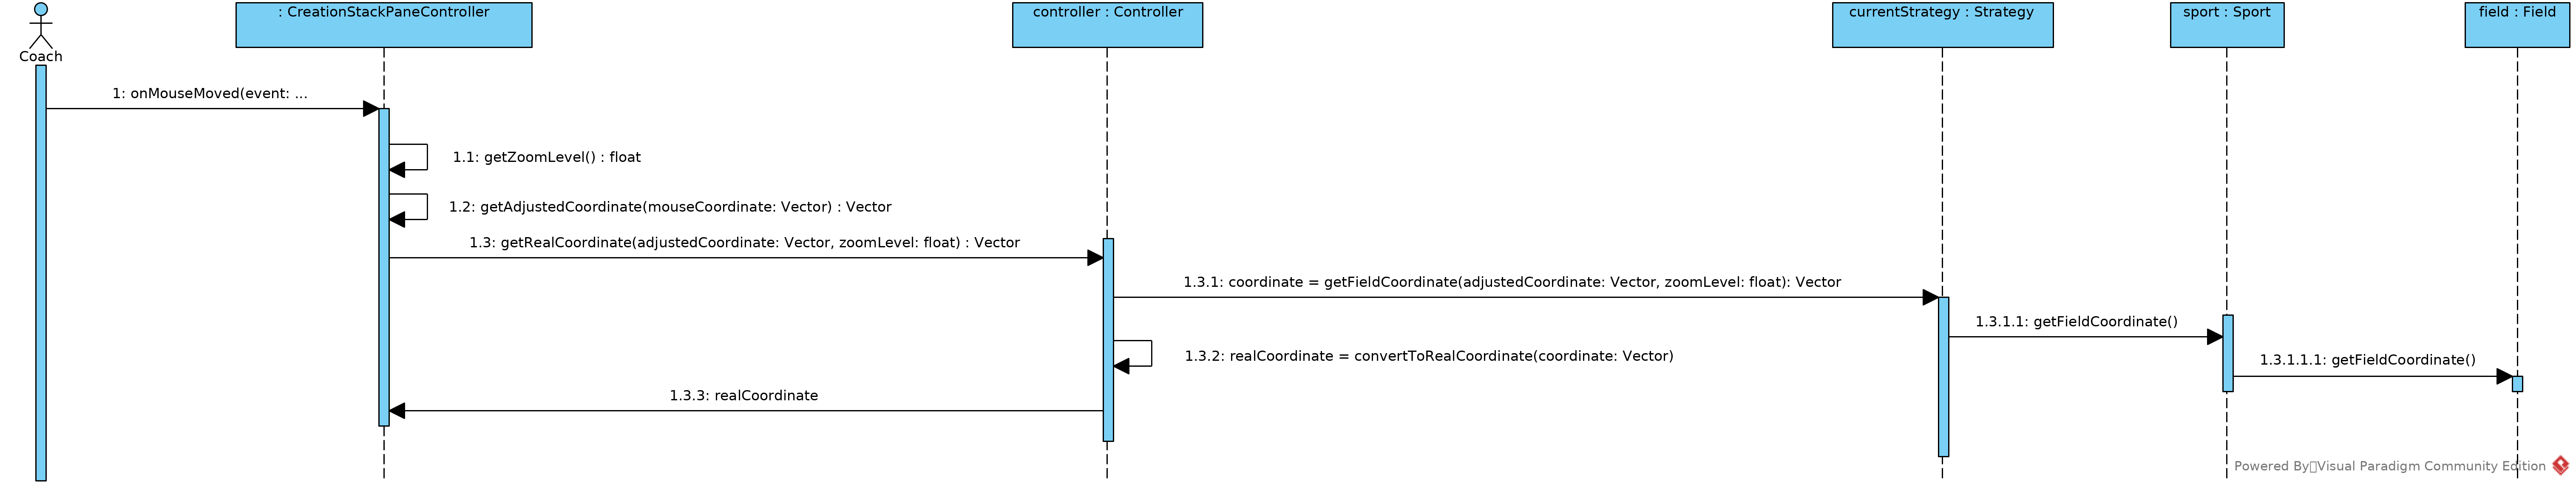
\includegraphics[scale=0.7]{fig/dsc_getRealCoordinate.png}
%    \caption{Diagramme de séquence de conception pour Convertir les coordonnées de la souris en coordonnées réelles}
%    \label{fig:dsc_pixel_reel}
%\end{figure}

La figure \ref{fig:dsc_pixel_reel} est le diagramme de séquence pour obtenir les coordonées réelles à partir des coordonnées de la souris.
La fenêtre reçois un événement lors du déplacement de la souris.
Elle récupère le niveau de zoom actuel et ajuste les coordonnées de la souris selon le déplacement horizontal et vertical du terrain.
Le contrôleur est appelé, qui délègue l'appel pour obtenir les coordonées du terrain à la stratégie courante.
Une fois les coordonnées du terrain obtenues, elles sont converties en coordonnées réelles (e.g: en mètre) et retournées.


\section{Ajouter un joueur}
\label{sec:ajouter_joueur}

%\begin{figure}[htpb]
%    \centering
%    \includegraphics[scale=0.7]{fig/dsc_createPlayer.png}
%    \caption{Diagramme de séquence de conception pour ajouter un joueur sur le terrain}
%    \label{fig:dsc_create_player}
%\end{figure}

La figure \ref{fig:dsc_create_player} est le diagramme séquence lorsqu'un nouveau joueur est ajouté sur le terrain.

%\begin{figure}[htpb]
%    \centering
%    \includegraphics[scale=0.7]{fig/dsc_dragPlayer.png}
%    \caption{Diagramme de séquence de conception pour déplacer un joueur sur le terrain}
%    \label{fig:dsc_drag_player}
%\end{figure}

La figure \ref{fig:dsc_drag_player} est le diagramme de séquence lorqu'un joueur est déplacé à un nouvel endroit sur le terrain.

\section{Sélectionner l'objet de jeu sous la souris après un clic}
\label{sec:convertir_clic_en_objet}

%\begin{figure}[htpb]
%    \centering
%    \includegraphics[scale=0.7]{fig/dsc_getGameObject.png}
%    \caption{Diagramme de séquence de conception pour obtenir l'objet de jeu sous la souris après un clic}
%    \label{fig:dsc_get_game_object}
%\end{figure}

La figure \ref{fig:dsc_get_game_object} est le diagramme de séquence pour sélectionner l'objet de jeu sous la souris.
Les coordonnées du terrain sont obtenus en délégant l'appel à la stratégie courante.
L'image actuelle de la stratégie est récupérée et l'objet \textit{Frame} est appelée.
Celui-ci parcours tous les objets de jeu qu'il contient et calcul la distance entre les coordonnées et l'objet de jeu.
Si la distance est inférieur aux valeurs de dimensions en x ou en y, l'id de cet objet de jeu est retourné.
Autrement, un id \textit{null} est retourné.

\section{Édition en mode image par image}
\label{sec:edition_image_par_image}

%\begin{figure}[htpb]
%    \centering
%    \includegraphics[scale=0.7]{fig/dsc_editImageByImage.png}
%    \caption{Diagramme de séquence de conception pour le mode d'édition image par image}
%    \label{fig:dsc_edit_image}
%\end{figure}

La figure \ref{fig:dsc_edit_image} est le diagramme de séquence des différentes intéractions entre le système et l'utilisateur lors de l'édition d'une stratégie en mode \textbf{image par image}.
Lorsque l'utilisateur change pour ce mode d'édition, la fenête principale s'occupe d'initialiser les éléments de la vue.
Si l'utilisateur clic sur un joueur et le déplace, les scénarios pour obtenir la sélection sous la souris \ref{sec:convertir_clic_en_objet} et déplacer un joueur \ref{sec:ajout_joueur} sont exécutés.
Par soucis de lisibilités, tous les appels ne sont pas reproduit.

Lorsque l'utiliseur clic sur «prochaine image», la fenêtre sauvegarde les informations actuels et appel le contrôleur pour obtenir la prochaine image.
S'il n'y a pas de prochaine image, une nouvelle est créée en copiant les informations de celle actuelle.
La vue rend transparent les informations de l'ancienne image et affiche la nouvelle image.

Lorsque l'utilisateur clic sur «image précédente», la fenêtre récupère à l'aide du contrôleur les deux dernières images.
Si une des deux images n'existe pas, null est retournée.
La plus ancienne des deux images est affichée avec un niveau de transparence et l'image immédiatement précédente à celle encours est affichée.

Si l'utilisateur est en mode «suppresion», lorsqu'il clic sur un objet de jeu, le scénario pour obtenir la sélection, \ref{sec:convertir_clic_en_objet} est exécuté.
Un appel au contrôleur est fait pour supprimer l'objet avec l'identifiant acquis.
Cet appel est uniquement exécuté si l'identifiant n'est pas null.

\section{Édition en mode temps réel}
\label{sec:edition_temps_reel}

%\begin{figure}[htpb]
%    \centering
%    \includegraphics[scale=0.7]{fig/dsc_editRealTime.png}
%    \caption{Diagramme de séquence de conception pour le mode d'édition en temps réel}
%    \label{fig:dsc_edit_real_time}
%\end{figure}

La figure \ref{fig:dsc_edit_real_time} est le diagramme de séquence des différentes intéractions entre le système et l'utilisateur lors de l'édition d'une stratégie en mode \textbf{temps réel}.
Ce mode est très similaire avec celui image par image (\ref{sec:edition_impage_par_image}).
La différence principale est que lorsque l'utilisateur exécute le scénario pour déplacer un joueur (\ref{sec:ajout_joueur}), plusieurs appels supplémentaires doivent être faits.
Lorsqu'un déplacement est débuté, un booléen est modifié à Vrai.

À chaque événement de déplacement de la souris, les appels nécessaires pour positionner le joueur sont faits.
Plutôt que de positionner dans une image, la position est mise dans une \textbf{sous-image}.
Cette sous-image est retournée et affichée.
Ceci permet de rejouer les mouvements depuis la dernière image des joueurs.

Lorsque le déplacement est terminé, la fenêtre met fin au mode de déplacement en temps réel.
L'édition en temps réel peut se poursuivre.

\section{Visionner le jeu}
\label{sec:visionner_jeu}

%\begin{figure}[htpb]
%    \centering
%    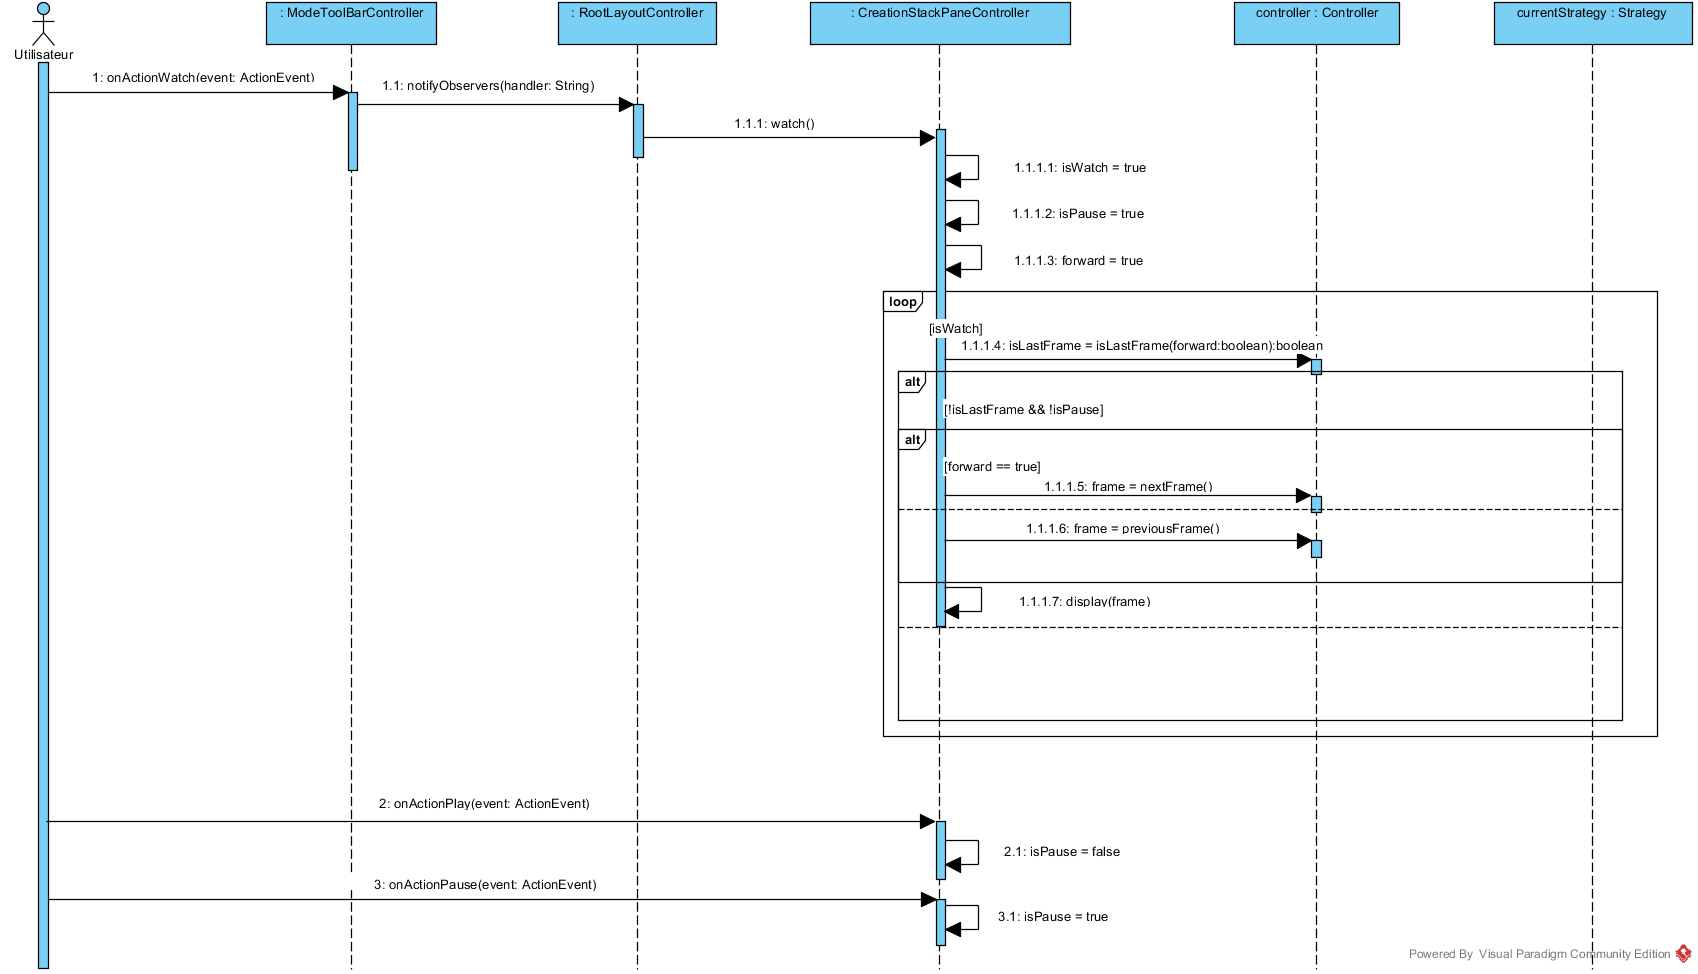
\includegraphics[scale=0.7]{fig/dsc_visionnement_watch.png}
%    \caption{Diagramme de séquence de conception pour le mode de visionnement (partie principale)}
%    \label{fig:dsc_view_main}
%\end{figure}

La figure \ref{fig:dsc_view_main} est le diagramme de séquence pour les principales intéractions lors du visionnement.

Lorsque l'utilisateur passe en mode visionnement, le système entre dans une boucle gouverné par un booléen: \textbf{isWatch}.
Par défaut, le visionnement est sur pause.
Si l'utilisateur active le visionnement, le booléen: \textbf{isPause} est mis à Faux.
Si l'utilisateur met sur pause, ce même booléen est mis à Vrai.
À chaque itération de la boucle, le système récupère une image et l'affiche s'il n'est pas sur pause ou si la dernière image affichée n'était pas la dernière image disponible.

%\begin{figure}[htpb]
%    \centering
%    \includegraphics[scale=0.7]{fig/dsc_visionnement_edit_index.png}
%    \caption{Diagramme de séquence de conception pour le mode de visionnement (modification du temps)}
%    \label{fig:dsc_view_edit_idx}
%\end{figure}

La figure \ref{fig:dsc_view_edit_idx} est le diagramme de séquence lorsque l'utilisateur souhaite avancer ou reculer d'un temps ajustable.
Lorsque le temps est saisie, le système appel le contrôleur pour ajuster le temps actuel.
Le contrôleur est responsable de traduire le différentiel de temps en un différentiel d'images et il tente de modifier autant que possible l'image en cours.
La nouvelle image actuelle est retournée et affichée.

%\begin{figure}[htpb]
%    \centering
%    \includegraphics[scale=0.7]{fig/dsc_visionnement_forward.png}
%    \caption{Diagramme de séquence de conception pour le mode de visionnement (avancement rapide)}
%    \label{fig:dsc_view_forward}
%\end{figure}

La figure \ref{fig:dsc_view_forward} est le diagramme de séquence lorsque l'utilisateur souhaite avancer en accélérer la stratégie.
Le sens est vérifié et si le visionnement se faisait en reculant, la vitesse de visionnement est remise à sa valeur par défaut.
La vitesse est accélérée en appelant le contrôleur.

%\begin{figure}[htpb]
%    \centering
%    \includegraphics[scale=0.7]{fig/dsc_visionnement_rewind.png}
%    \caption{Diagramme de séquence de conception pour le mode de visionnement (reculuement rapide)}
%    \label{fig:dsc_view_rewind}
%\end{figure}

La figure \ref{fig:dsc_view_rewind} est le diagramme de séquence lorsque l'utilisateur souhaite reculer en accélérer la stratégie.
C'est la même logique que dans le cas de l'avancement rapide, mais modifié pour tenir compte du sens de visionnement renversé.


% Annexes
\appendix
%!TEX encoding = UTF-8 Unicode
% -*- coding: UTF-8; -*-
% vim: set fenc-utf-8
%

\chapter{Échéancier}
\label{s:echeancier}

L'image de l'\'ech\'eancier est disponible sous \textit{/rapport/fig/echeancier.png}.

\begin{figure}[htpb]
    \centering
    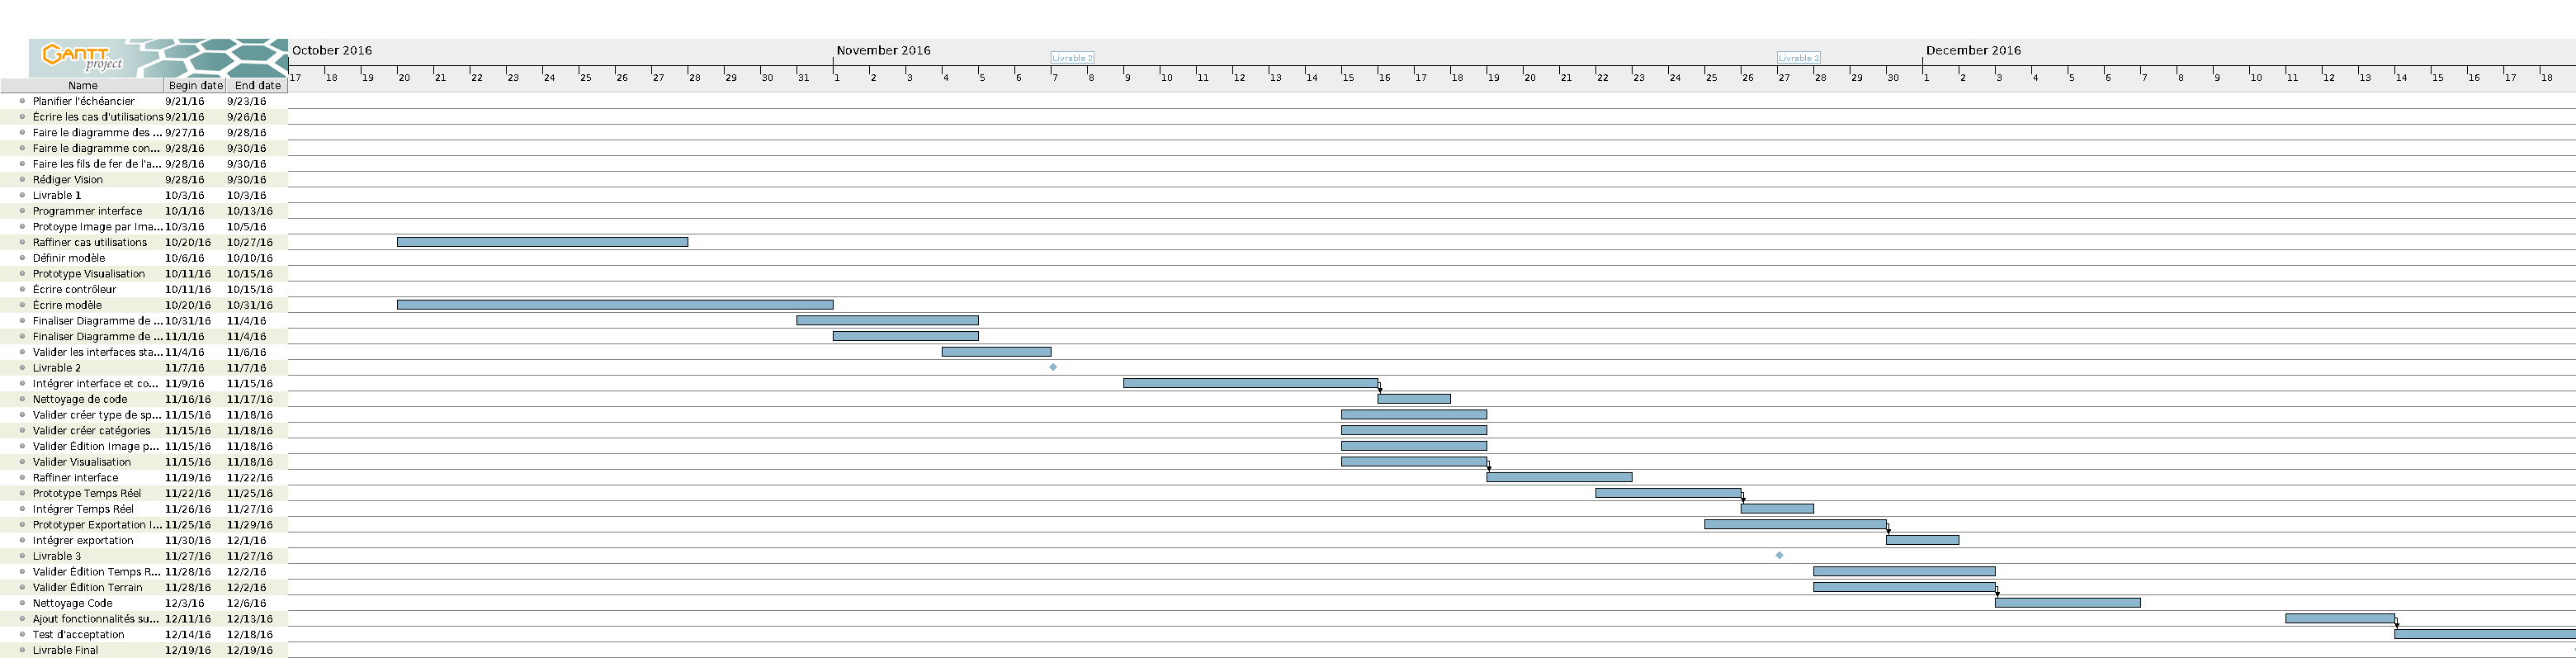
\includegraphics[scale=0.29, angle=90]{fig/echeancier.png}
    \caption{Gantt pour la planification du projet}
    \label{fig:echeancier}
\end{figure}

%!TEX encoding = UTF-8 Unicode
% -*- coding: UTF-8; -*-
% vim: set fenc-utf-8

\chapter{Vision}
\label{s:vision}

Suite à une rencontre avec le président de l'AEMQ (Association des entraîneurs mineurs du Québec), notre \textbf{jeune pousse} s'est vu confier le mandat de réaliser l'application VisuaLigue, qui a pour objectif de simplifier l'enseignement des stratégies de jeu pour les entraîneurs.
Cette application doit permettre aux entraîneurs de créer facilement des stratégies, puis de les présenter de façon dynamique et en temps réel aux joueurs.

La cr\'eation des strat\'egies s'effectue en dessinant les s\'eries d'actions que les joueurs doivent ex\'ecuter.
Un entraîneur peut créer une nouvelle stratégie ou modifier une stratégie existante.
La création d'une stratégie nécessite que chaque joueur ait sa série d'actions.
Pour cela, il faut s\'electionner un joueur, lui assigner un r\^ole et dessiner ensuite les actions qu'il doit faire.
Quand une strat\'egie est compl\'et\'ee, il est possible de la sauvegarder et de l'exporter.
Un utilisateur, que ce soit un entraîneur ou un joueur, peut visualiser une strat\'egie pr\'ec\'edemment d\'efinie.
Lors de la visualisation, il est possible d'arr\^eter, de red\'emarrer, d'avancer ou de reculer le visionnement.
De plus, plusieurs sports peuvent \^etre d\'efinis.
L'entraîneur peut aussi créer un nouveau sport ou en modifier un existant.
Il peut ainsi sp\'ecifier un terrain, un projectile et des r\^oles pour un sport.
La création d'un terrain se fait de deux façons: en important une image représentant le terrain ou en dessinant les lignes via l'application.
Pour les deux cas, il faut que les dimensions du terrain soient spécifiées.

L'application permet d'obtenir des strat\'egies que l'utilisateur peut visualiser en temps r\'eel.
Puisque la visualisation des stratégies décrites par un entraîneur est le but principal, il est primordial que l\'utilisation de l\'application soit naturelle et que son interface ne soit pas surchargée.

%!TEX encoding = UTF-8 Unicode
% -*- coding: UTF-8; -*-
% vim: set fenc-utf-8

\chapter{Maquette des interfaces}
\label{s:maquettes_interfaces}

Ce chapitre présente les maquettes des principales interfaces de l'application VisuaLigue.
Une courte explication des fonctionnalités moins évidentes est également présente à la suite des figures si nécessaire.

\begin{figure}[htpb]
    \centering
    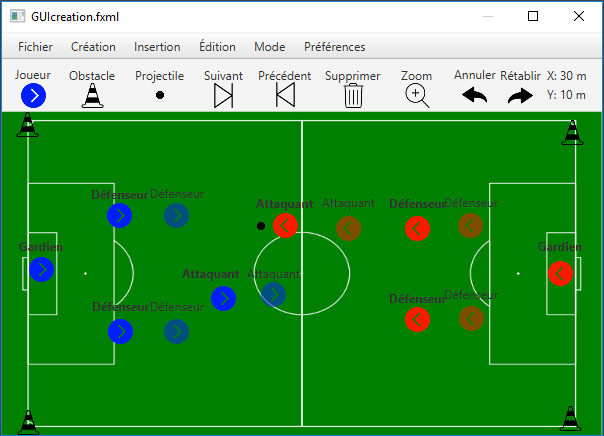
\includegraphics[scale=0.6]{fig/gui/gui_creation.png}
    \caption{Interface pour la création des stratégies}
    \label{fig:gui:gui_creation}
\end{figure}

L'interface \ref{fig:gui:gui_creation} permet l'édition des stratégies, soit en mode image par image ou en mode temps réel.
Les trois premiers icônes en partant de la gauche permettent de glisser des éléments sur le terrain.
Les icônes "suivant" et "précédent" permettent respectivement d'avancer ou de reculer d'une image dans le mode image par image.
Les étiquettes "x" et "y" à la droite des icônes correspondent aux coordonnées de la souris sur le terrain en unités réelles.
La transparence de certains joueurs sur la figure ci-dessus correspond à des éléments qui proviennent d'une image précédente lors de l'édition en mode image par image.

\begin{figure}[htpb]
    \centering
    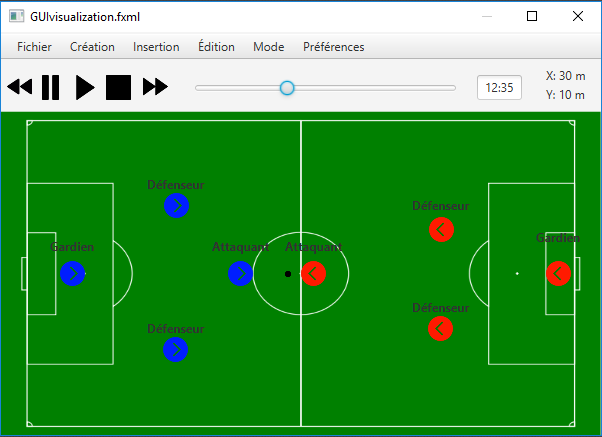
\includegraphics[scale=0.6]{fig/gui/gui_visualisation.png}
    \caption{Interface pour la visualisation des stratégies}
    \label{fig:gui:gui_visualisation}
\end{figure}

L'interface \ref{fig:gui:gui_visualisation} permet la visualisation des stratégies préalablement créées.
En plus des boutons habituels de visionnement de vidéos, on y retrouve un curseur glissant permettant de se déplacer facilement à n'importe quel temps de la stratégie.
Ce temps peut aussi être modifié directement dans la boîte de saisie prévue à cet effet à la droite du curseur.
Les coordonnées de la souris sont encore affichées.

\begin{figure}[htpb]
    \centering
    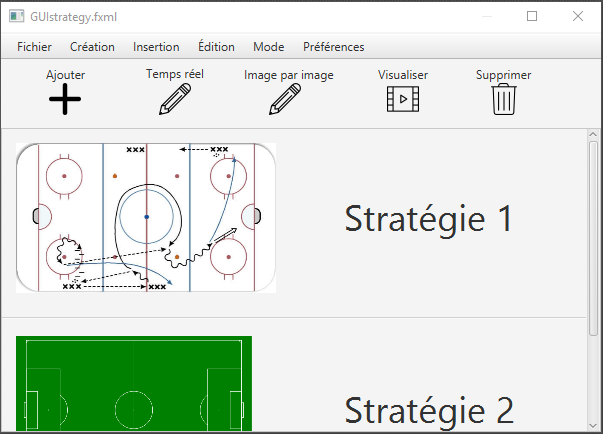
\includegraphics[scale=0.6]{fig/gui/gui_strategie.png}
    \caption{Interface de gestion des stratégies}
    \label{fig:gui:gui_strategie}
\end{figure}

L'interface \ref{fig:gui:gui_strategie} permet la gestion des stratégies.
Après avoir sélectionné une stratégie, une multitude de choix s'offre à l'entraîneur.
Il peut supprimer la stratégie, la visionner, ou bien l'éditer soit en mode temps réel ou en mode image par image.
Bien sûr, l'interface permet aussi l'ajout d'une nouvelle stratégie.
\newpage

\begin{figure}[htpb]
    \centering
    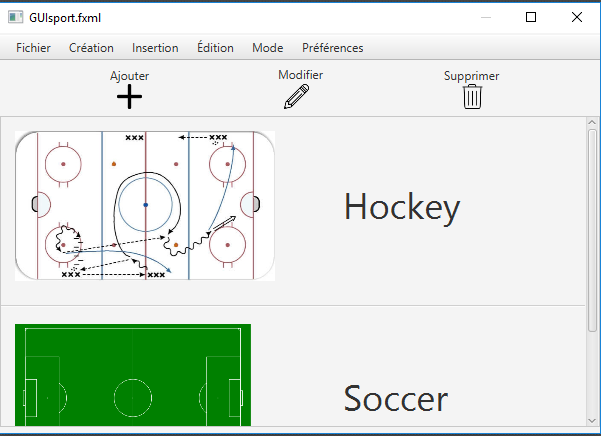
\includegraphics[scale=0.6]{fig/gui/gui_sport.png}
    \caption{Interface de gestion des sports}
    \label{fig:gui:gui_sport}
\end{figure}

L'interface \ref{fig:gui:gui_sport} permet la gestion des sports.
Il est possible d'ajouter, de modifier ou de supprimer un sport.

\begin{figure}[htpb]
    \centering
    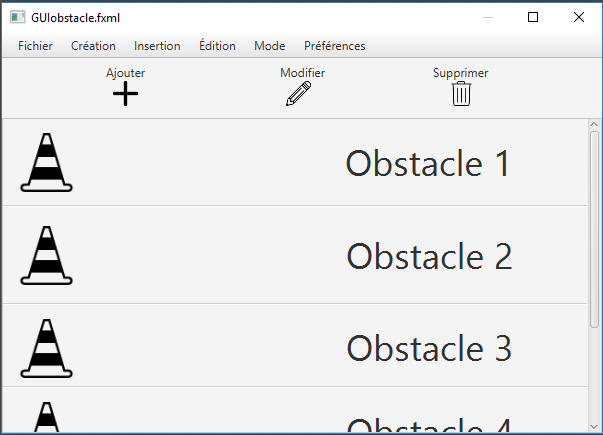
\includegraphics[scale=0.6]{fig/gui/gui_obstacles.png}
    \caption{Interface de gestion des obstacles}
    \label{fig:gui:gui_obstacles}
\end{figure}

L'interface \ref{fig:gui:gui_obstacles} permet la gestion des obstacles.
Les fonctionnalités sont les mêmes que pour la gestion des stratégies.

\newpage

\begin{figure}[htpb]
    \centering
    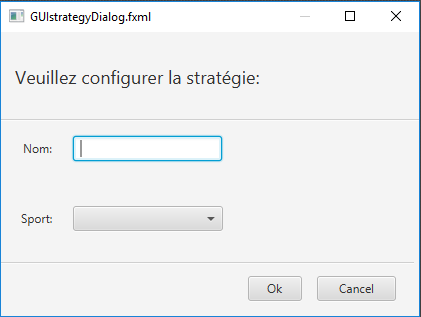
\includegraphics[scale=0.6]{fig/gui/gui_strategie_dialog.png}
    \caption{Interface de configuration des stratégies}
    \label{fig:gui:gui_strategie_dialog}
\end{figure}

La fenêtre de dialogue \ref{fig:gui:gui_strategie_dialog} permet de configurer une stratégie.
Elle apparaît lorsque l'on modifie ou ajoute une stratégie via la fenêtre de gestion des stratégies.
On y retrouve une boîte de saisie pour le nom de la stratégie et une boîte de choix pour y associer un sport préalablement créé.

\begin{figure}[htpb]
    \centering
    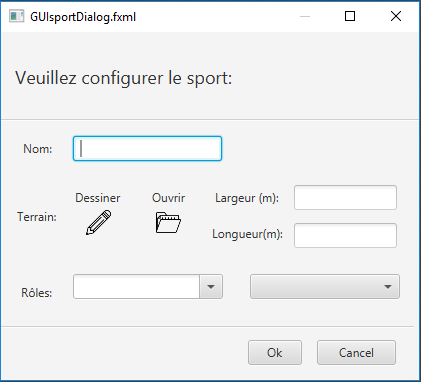
\includegraphics[scale=0.6]{fig/gui/gui_sport_dialog.png}
    \caption{Interface de configuration des sports}
    \label{fig:gui:gui_sport_dialog}
\end{figure}

La fenêtre de dialogue \ref{fig:gui:gui_sport_dialog} permet de configurer un sport.
Elle apparaît lorsque l'on modifie ou ajoute un sport via la fenêtre de gestion des sports.
On y retrouve entre autres deux icônes pour dessiner le terrain ou choisir une image déjà existante.
Deux autres champs permettent la saisie des dimensions réelles du terrain.
Finalement, on peut créer ou choisir un rôle parmi ceux déjà créés afin d'établir la liste des catégories de joueur pour le sport.

\newpage

\begin{figure}[htpb]
    \centering
    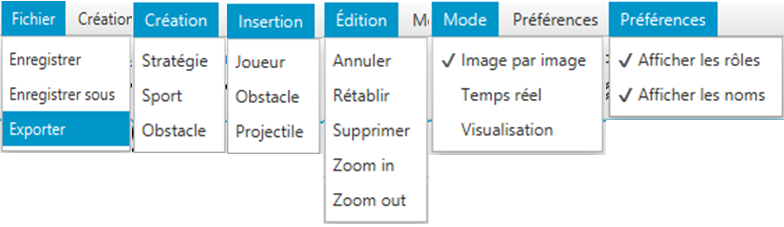
\includegraphics[scale=0.7]{fig/gui/gui_menu.png}
    \caption{Interface du menu pour montrer les options}
    \label{fig:gui:gui_menu}
\end{figure}

La figure \ref{fig:gui:gui_menu} montre toutes les options du menu présent dans les principales interfaces.
La majorité des fonctionnalités du logiciel sont accessibles par ce menu.
Il est important de comprendre que le sous-menu "mode" ne permet pas le choix de plus d'une option à la fois, contrairement au sous-menu préférences.

%!TEX encoding = UTF-8 Unicode
% -*- coding: UTF-8; -*-
% vim: set fenc-utf-8

\chapter{Modèle du domaine}
\label{s:modele_domaine}

%!TEX encoding = UTF-8 Unicode
% -*- coding: UTF-8; -*-
% vim: set fenc-utf-8

\chapter{Cas d'utilisations}
\label{s:cas_utilisation}

Ce chapitre présente les différents cas d'utilisation pour l'application VisuaLigue.
La figure \ref{fig:cas_utilisation_diag} résume les acteurs du systèmes et les cas d'utilisations.
La suite du chapitre décrie en détails les cas d'utilisations et s'attarde sur les plus importants.

\begin{figure}[htpb]
    \centering
    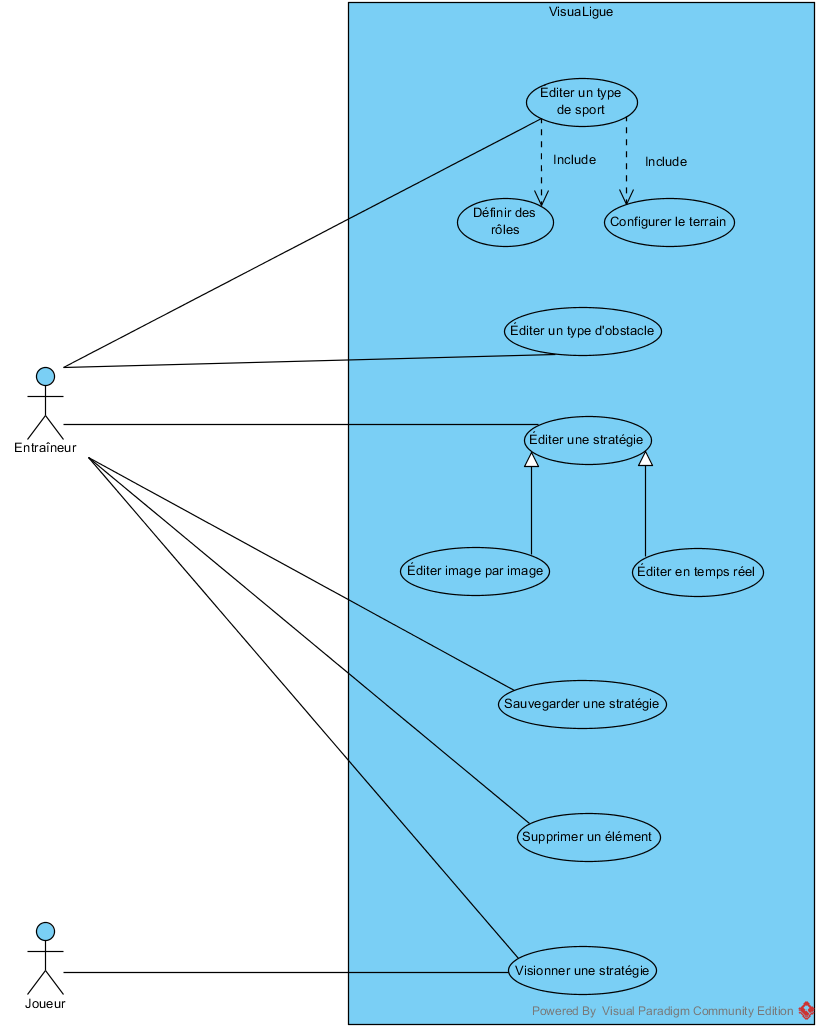
\includegraphics[scale=0.7]{fig/cas_utilisation_diag.png}
    \caption{Diagramme des cas d'utilisations}
    \label{fig:cas_utilisation_diag}
\end{figure}

\newpage

\section{Ajouter un type de sport}
\label{sec:ajouter_un_type_de_sport}

\subsection{Sc\'enario principal}
\label{sub:sc'enario_principal}

L'entra\^ineur cr\'ee un sport, le nomme.
Ensuite il ajoute les r\^oles du sport.
Finalement, il d\'efini un terrain en dessinant les lignes et en sp\'ecifiant les dimensions.

\subsection{Autres Situations}
\label{sub:autres_situations}
\begin{itemize}
    \item \textbf{Sport d\'ej\`a existant:} Si le sport existe d\'ej\`a dans l'application, un message d'avertissement appara\^it pour signaler que le sport existe d\'ej\`a. 
    L'entraîneur peut d\'ecider d'effacer ce qui \'etait dans le sport existant, d'enregister son sport sous un autre nom, ou d'oublier le sport cr\'e\'e. 
\end{itemize}

\section{Ajouter une stratégie}
\label{sec:ajouter_une_strategie}

\subsection{Pr\'erequis}
\label{sub:prerequis}

Le sport pour lequel l'entraîneur veut ajouter une stratégie doit exister dans l'application.

\subsection{Sc\'enario principal}
\label{sub:sc'enario_principal}

L'entraîneur veut ajouter une nouvelle stratégie.
Il choisi le sport pour la strat\'egie.
Ensuite, pour chacun des joueurs, il leur assigne un r\^ole et dessine leurs actions.

\subsection{Autres Situations}
\label{sub:autres_situations}
\begin{itemize}
    \item \textbf{Sport d\'ej\`a existant:} Si la stratégie existe d\'ej\`a dans l'application, un message d'avertissement appara\^it pour signaler que celui-ci existe d\'ej\`a. 
    L'entraîneur peut d\'ecider d'effacer ce qui \'etait dans la stratégie existante, d'enregister sa stratégie sous un autre nom, ou d'oublier la stratégie cr\'e\'e. 
\end{itemize}

\section{Visualiser une stratégie}
\label{sec:visualiser_une_strategie}

\subsection{Pr\'erequis}
\label{sub:prerequis}
Il faut que la strat\'egie soit enregistr\'ee dans l'application pour que l'entraîneur puisse la visualiser.

\subsection{Sc\'enario principal}
\label{sub:sc'enario_principal}

L'\textit{entra\^ineur} s\'electionne la \textit{strat\'egie} \`a visualiser.
Il d\'ebute la visualisation et observe le d\'eroulement de la \textit{strat\'egie}.
Il peut mettre fin \`a la visualisation \`a tout moment.

\section{Exporter une stratégie}
\label{sec:exporter_une_strategie}

\subsection{Pr\'erequis}
\label{sub:prerequis}
Il faut que la strat\'egie soit enregistr\'ee dans l'application pour que l'entraîneur puisse l'exporter.

\subsection{Sc\'enario principal}
\label{sub:sc'enario_principal}

L' \textit{entra\^ineur} veut exporter une strat\'egie.
Il s\'electionne la strat\'egie et le format pour l'exportation.
Il applique l'exportation de la strat\'egie.

%!TEX encoding = UTF-8 Unicode
% -*- coding: UTF-8; -*-
% vim: set fenc-utf-8
%

\chapter{Glossaire}
\label{s:glossaire}

\begin{itemize}
    \item Action: Déplacement ou interaction avec le projectile d'un joueur.
        \\
    \item Entra\^ineur: Utilisateur qui construit une strat\'egie et la pr\'esente \`a des joueurs.
        \\
    \item Joueur: Utilisateur qui ex\'ecute une action et qui poss\`ede un r\^ole.
        \\
    \item Obstacle: Objet statique qu'un joueur doit \'eviter lors d'un d\'eplacement.
        \\
    \item Projectile: Objet principal d'un sport, \textit{e.g:} balle, ballon, rondelle, etc.
        \\
    \item R\^ole: Fonction d'un joueur lors d'une strat\'egie, \textit{e.g:} ailier, centre, d\'efenseur, etc.
        \\
    \item Stratégie: Ensemble des s\'equences des actions des joueurs.
        \\
\end{itemize}

%!TEX encoding = UTF-8 Unicode
% -*- coding: UTF-8; -*-
% vim: set fenc-utf-8
%

% Ordre alphabétique selon la ref bibitem
\begin{thebibliographyUL}{99}
    %Enonce de projet
    \bibitem{enonce} Jonathan Gaudreault, Martin Savoie, 2016, \emph{Énoncé de projet: VisuaLigue}, Département d'informatique et de génie logiciel de l'Université Laval, 4 p.
\end{thebibliographyUL}

\end{document}
% Fin du document
